% !TEX root = ../main.tex
%
\chapter{Background}
\label{sec:background}

\section{View Synthesis}

View synthesis is a computer graphics and computer vision process that involves the creation of new, synthetic images of a scene from viewpoints that were not originally captured by a camera. This technique leverages existing images and often incorporates geometric information about the scene, enabling the generation of perspective-correct views from desired locations.
The objective of view synthesis is to generate realistic and accurate representations of a 3D scene from novel viewpoints, thereby enhancing applications such as virtual reality (VR), augmented reality (AR), 3D television, and film production. The following sections provide an overview of traditional view synthesis techniques.

\paragraph{Image-Based Rendering Techniques}
Image-based rendering (IBR) techniques focus on synthesizing new views of a scene using pre-captured images, with minimal reliance on geometric models.
The fundamental principle of IBR is to directly utilize the radiance information captured in these images, manipulating it to generate new viewpoints without the necessity for detailed 3D reconstruction.
This approach is particularly advantageous in scenarios where fast rendering is necessary or when accurate geometric data is unavailable.
IBR methods are distinguished by their capacity to generate photorealistic results, as they accurately capture lighting, shadows, and reflections in accordance with the original scene.
These methods, such as those employing light fields or lumigraphs, are particularly suited to applications where visual realism is of critical importance, as they are able to efficiently simulate the complexity of real-world lighting and textures \cite{buehler_unstructured_2001,chen_view_1993,debevec_modeling_1996,gortler_lumigraph_1996,levoy_light_1996}.

\paragraph{Volumetric Methods}
Volumetric rendering techniques construct a 3D volume of the scene, often represented as a grid of voxels. Each voxel contains data such as color and opacity, which contribute to the final image through a process akin to 3D texturing. Unlike surface-based modeling, which requires explicit surfaces, volumetric methods fill the entire data space, allowing for the handling of complex phenomena like fog, clouds, and fire, which do not have clear boundaries.
This approach is advantageous when the scene involves intricate details and volumetric phenomena that traditional polygon-based rendering might struggle to capture accurately. Volumetric methods often employ techniques such as voxel coloring to integrate multiple images into a cohesive 3D model \cite{curless_volumetric_1996,seitz_photorealistic_1999}.

\todo{expand and include figures}

\section{Neural Approaches to View Synthesis}
Neural approaches to view synthesis have significantly advanced the capabilities of generating realistic views from sparse data.
These methods integrate deep learning techniques to enhance the synthesis process, offering substantial improvements over traditional geometric and image-based methods.

\paragraph{Deep Learning for View Synthesis}
Deep learning models, particularly Convolutional Neural Networks (CNNs), are employed to predict depth and color information from sparse sets of images.
These models facilitate the synthesis of intermediate views by interpolating between captured viewpoints, efficiently handling scenarios with incomplete data where traditional methods would struggle \cite{kalantari_learning-based_2016,maxim_tatarchenko_single-view_2015,peter_hedman_deep_2019}.

\paragraph{Learning Volumetric Representations}
Recent advances in neural view synthesis have explored volumetric representations as a means of effectively encoding 3D scene information.
This approach employs deep learning to construct volumetric grids or embeddings that capture both color and spatial data, thereby enabling dynamic and realistic rendering of new views.
Such volumetric techniques represent a significant departure from traditional modeling, as they provide a framework where 3D features are embedded directly into the network. This enables sophisticated scene understanding and rendering without the need for explicit geometric reconstruction \cite{lombardi_neural_2019,sitzmann_deepvoxels_2019}.

\paragraph{Multiplane Images and Scene Representation}
Multiplane Images (MPIs) represent a neural approach to view synthesis, whereby scenes are decomposed into layers at different depths.
Neural networks are capable of creating these layered representations from a limited number of views.
Subsequently, the learned MPIs can be efficiently re-rendered from new perspectives using traditional graphics techniques.
This method provides a robust solution for generating photorealistic and geometrically coherent views by accommodating variations in scene complexity and effectively handling occlusions. \cite{mildenhall_local_2019,penner_soft_2017,pratul_p_srinivasan_pushing_2019,tao_zhou_stereo_2018}.

\paragraph{End-to-End Learning}
The advent of end-to-end learning with deep neural networks has significantly simplified the view synthesis process. This is due to the fact that a single network is now capable of handling multiple synthesis tasks concurrently.
This approach reduces the complexity and potential failure points associated with multi-stage synthesis methods.
The training of these networks on large datasets of posed imagery enables them to learn complex mappings from input images to synthesized views, efficiently handling challenging scenarios \cite{chen_photographic_2017,flynn_deep_2016}.

\section{Neural Radiance Fields for View Synthesis}

Neural Radiance Fields (NeRF) offer a novel approach to view synthesis that significantly advances previous techniques.
Utilizing a fully connected deep neural network, NeRF optimizes a continuous volumetric scene function from a sparse set of input views \cite{mildenhall_nerf_2021}.
This method diverges from traditional discrete representations like voxel grids or mesh geometries, employing a more fluid and detailed scene representation.

\paragraph{Implementation}
NeRF synthesizes views by querying a five-dimensional coordinate space—comprising spatial locations \((x, y, z)\) and viewing directions \((\theta, \phi)\) along camera rays \frefadd{fig:nerf-overview}{a}.
Classic volume rendering techniques are then applied to convert the output densities and colors into images.
At the core of this process lies a Multilayer Perceptron (MLP), a type of neural network characterized by layers of interconnected nodes which process input data sequentially from input to output.
The MLP in NeRF takes sampled 3D points and corresponding viewing directions as input and outputs the color and volume density  \frefadd{fig:nerf-overview}{b}.
This output is then composited into a 2D image using volume rendering techniques  \frefadd{fig:nerf-overview}{c}.
Because this rendering function is differentiable, NeRF uses gradient descent to minimize the difference between synthesized images and observed ground truth, optimizing the neural representation of the scene  \frefadd{fig:nerf-overview}{d}.

\begin{figure}[h!]
  \centering
  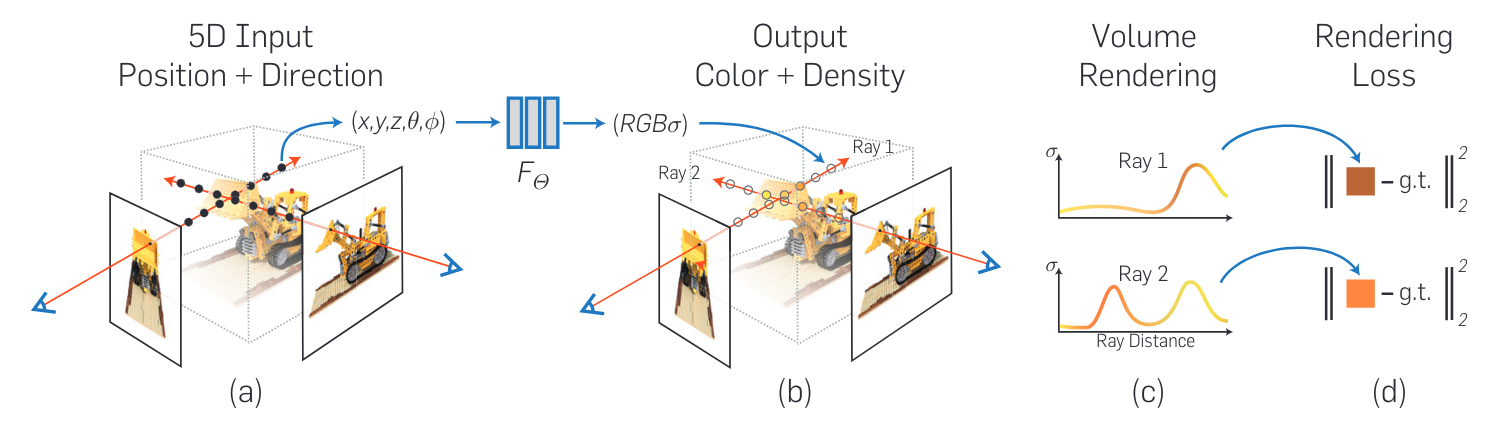
\includegraphics[width=\textwidth]{figures/bg-nerf.png}
  \caption{Overview of the NeRF scene representation and rendering procedure, illustrating the stages of sampling, neural processing, and image composition \cite{mildenhall_nerf_2021}.}
  \label{fig:nerf-overview}
\end{figure}

\paragraph{Advantages of NeRF}
In comparison to the methodologies previously discussed, NeRF offers a number of advantages.
It is capable of rendering high-resolution details and handling intricate geometries and material properties more effectively than mesh and voxel-based methods.
The continuous volumetric representation is not only capable of producing more photorealistic images but also remains highly efficient in memory usage.
This efficiency allows for the handling of complex real-world scenes without the storage and computation costs associated with traditional 3D representations.

\paragraph{Extensions and Applications of NeRF}
The landscape of NeRF has been expanded by several innovative extensions that enhance the utility and interactivity of NeRF models.
NeRF frameworks with user interfaces have emerged, enabling users to explore and manipulate 3D scenes \cite{muller_instant_2022,tancik_nerfstudio_2023}.
These frameworks provide features such as real-time scene rendering, adjustable training parameters, and the creation of camera trajectories for video rendering.
Recent advancements have introduced text-based manipulation, allowing users to edit and transform scenes through natural language descriptions \cite{bao_sine_2023,bar-tal_text2live_2022,haque_instruct-nerf2nerf_2023,jan-niklas_dihlmann_signerf_2024,wang_clip-nerf_2022}.
Another area of development is in color and appearance editing, where new methods enable adjustments of scene colors, consistent across varying views \cite{wu_palettenerf_2022}.
Additionally, some tools have integrated mesh editing capabilities, enhancing the geometric manipulation within NeRF-generated scenes \cite{yuan_nerf-editing_2022}.
These enhancements not only extend the functional range of NeRF but also significantly improve their application in creative industries.

In conclusion, NeRF's innovative use of neural networks for scene representation sets a new standard for photorealistic view synthesis, delivering high-quality results that are both computationally efficient and visually impressive.
